\documentclass[runningheads,a4paper]{llncs}

\usepackage{graphicx}
\usepackage{wrapfig}
\usepackage{subfigure}
\usepackage[utf8]{inputenc}
\pagenumbering{roman}
\usepackage{textcomp}
\usepackage{pifont}
\usepackage{color}
\usepackage{blindtext}
\usepackage{enumitem}


\begin{document}
\mainmatter  % start of an individual contribution

%Titel
\title{HCI Meilenstein 3}

\titlerunning{HCI Meilenstein 3}

\author{
  Dursun, Camkerten
  \texttt{a0027244@@unet.univie.ac.at}
  \and
  Pektas, Tarik
  \texttt{a1325165@@unet.univie.ac.at}
  \and
  Bozkurt Yigit Berkay
  \texttt{a1029659@@unet.univie.ac.at}
  \and
  Ayyildiz Mert Ahmet
  \texttt{a1125172@@unet.univie.ac.at}
}

\institute{Universität Wien  / HCI \\
\ SS16 / Gruppe 3 (Freitag) / Team 10}


\maketitle

\section{Farbliche Analyse}
Wir haben eine ähnliche Analyse schon vor der Implementierung gemacht und konnten bei der Farbwahl uns auf Farben beschränken welche auch von Farbblinden Menschen einwandfrei wahrgenommen werden können. Eine entsprechende Analyse in der wir den Color Blindness Simulator von Coblis verwendet haben bestätigte uns die von uns bereits erwarteten Resultate[1].\\ \\ 
Was allerdings leider nicht so gut funktioniert hat, war die Analyse der Reporting Seite da wir uns für eine Pie Chart entschieden hatten.\\\\ Da dieser sehr viele Farben, basierend auf unterschiedliche Datentypen hat, kann man da auch nicht viel ausrichten.\\ Dennoch haben wir, um den Informationsfluss auf jeden Fall zu gewähren, alternative Typen implementiert, wie zum Beispiel Table Chart oder Line Chart, welche die entsprechenden Farbanalysen bestanden haben und somit von jedem wahrgenommen werden können.

\begin{figure}
\centering
\subfigure[Normal Color Vision]{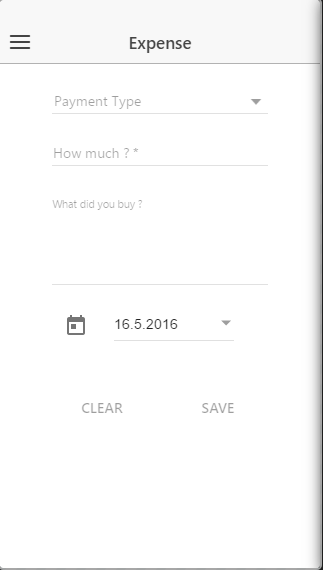
\includegraphics[width=0.15\textwidth]{expense.png}}
\hfill
\subfigure[Blue-Blind/Tritanopia]{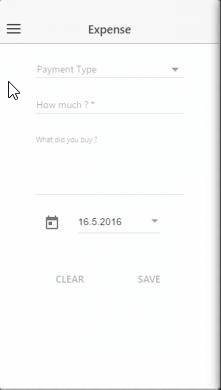
\includegraphics[width=0.15\textwidth]{expenseBlueBlind.png}}
\hfill
\subfigure[Green-Blind/Deuteranopia]{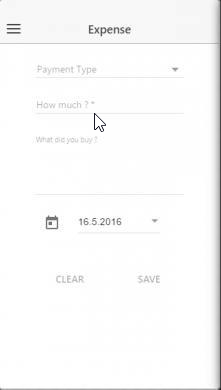
\includegraphics[width=0.15\textwidth]{expenseGreenBlind.png}}
\hfill
\subfigure[Red-Blind/Protanopia]{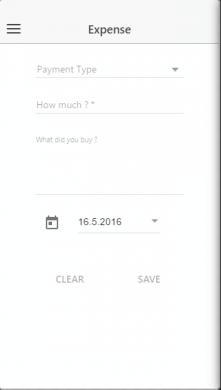
\includegraphics[width=0.15\textwidth]{expenseredblind.png}}
\end{figure}


\clearpage


\begin{figure}
\centering
\subfigure[Normal Color Vision]{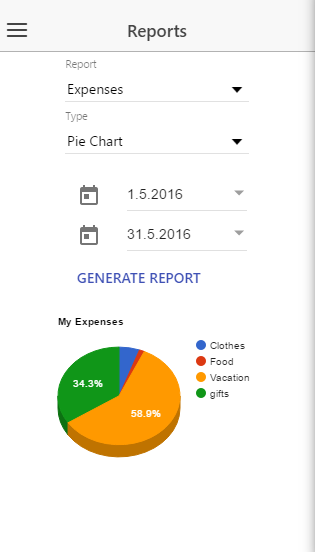
\includegraphics[width=0.15\textwidth]{ReportPieChart}}
\hfill
\subfigure[Blue-Blind/Tritanopia]{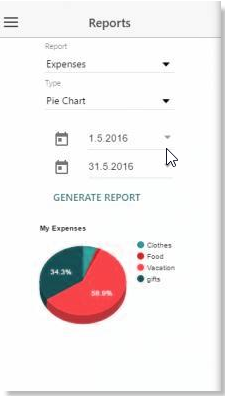
\includegraphics[width=0.15\textwidth]{ReportPieChartA2blueBlind.png}}
\hfill
\subfigure[Green-Blind/ Deuteranopia]{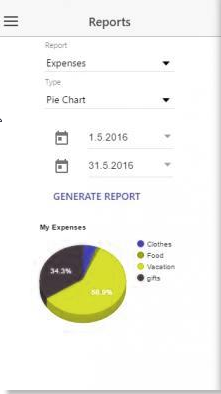
\includegraphics[width=0.15\textwidth]{ReportPieChartA2greenBlind.png}}
\hfill
\subfigure[Monochromacy/ Achromatopsia]{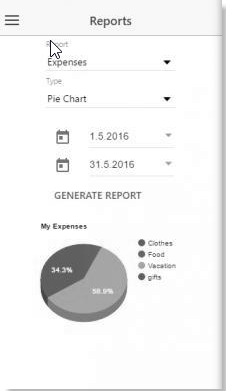
\includegraphics[width=0.15\textwidth]{ReportPieChartA2monochrom.png}}
\hfill
\subfigure[Red-Blind/Protanopia]{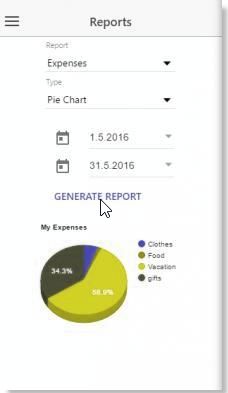
\includegraphics[width=0.15\textwidth]{ReportPieChartA2redBlind.png}}
\end{figure}

\begin{figure}
\centering
\subfigure[Normal Color Vision]{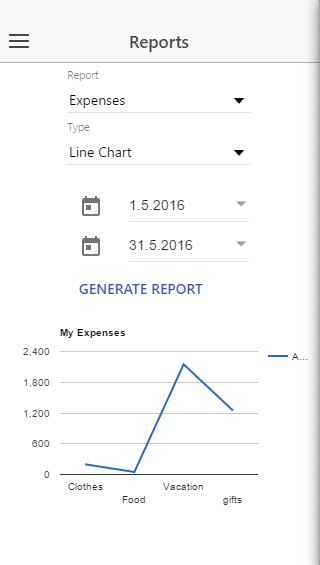
\includegraphics[width=0.15\textwidth]{LineChart.png}}
\hfill
\subfigure[Normal Color Vision]{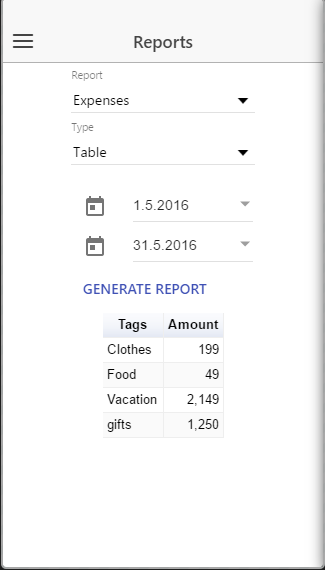
\includegraphics[width=0.15\textwidth]{tableChart.png}}
\hfill
\subfigure[Blue-Blind/Tritanopia]{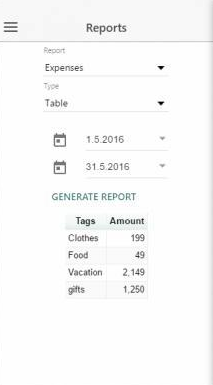
\includegraphics[width=0.15\textwidth]{tableChartBlueBlind.png}}
\hfill
\subfigure[Green-Blind/ Deuteranopia]{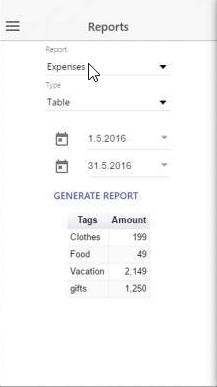
\includegraphics[width=0.15\textwidth]{tableChartGreenBlind.png}}
\hfill
\subfigure[Red-Blind/Protanopia]{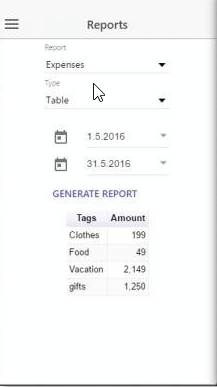
\includegraphics[width=0.15\textwidth]{tableChartRedBlind.png}}
\end{figure}


\section{Kognitive Analyse}

\subsection{Fitts Law und Hicks Law}

Wir haben versucht die gleichen Datentypen bzw Eingabefelder, wie zum Beispiel; Datum der Ausgabe; Startdatum für das Reporting, Datum der Einnahme etc. immer an die gleiche Stelle zu positionieren.\\\\  Dies galt natürlich auch für die restlichen Eingabefelder. Wir denken, dass wir somit eine Konsistenz in Bezug auf, häufig gesuchte Ziele an der gleichen Stelle, erstellen konnten. Bezüglich der Größe denken wir dass unsere Auswahl an Font und Size intuitiv bereits mit Fitts Law konform war.\\\\   Lag wahrscheinlich daran das bei Mobile Apps grundsätzlich Ziele des Öfteren sehr groß dargestellt werden. Wir beschlossen außerdem keine verschachtelten Menüstrukturen zur erstellen. \\\\ Alle wählbaren Optionen wurde in einzelnen Drop Down Menü Boxen erstellt.  Die Auswählbaren alternativen wurden in ihrer einfachsten Form, (Expense, Income, Report), formuliert. 


\begin{figure}
\centering
\subfigure[Expense]{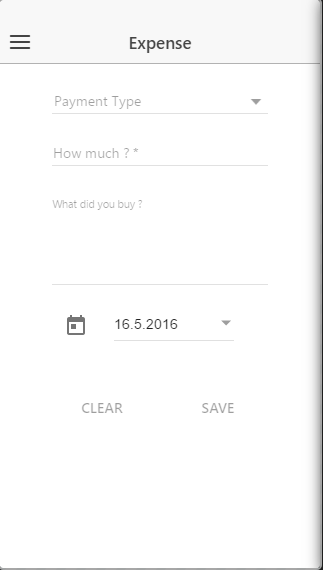
\includegraphics[width=0.15\textwidth]{expense.png}}
\hfill
\subfigure[Income]{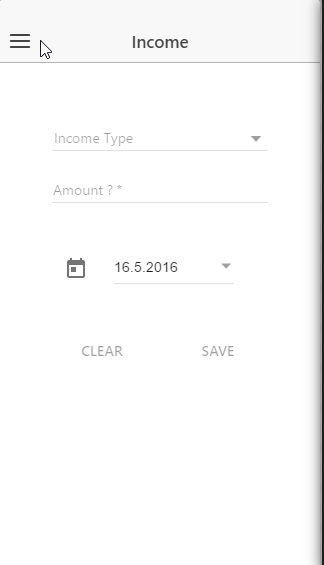
\includegraphics[width=0.15\textwidth]{income.png}}
\hfill
\subfigure[Report]{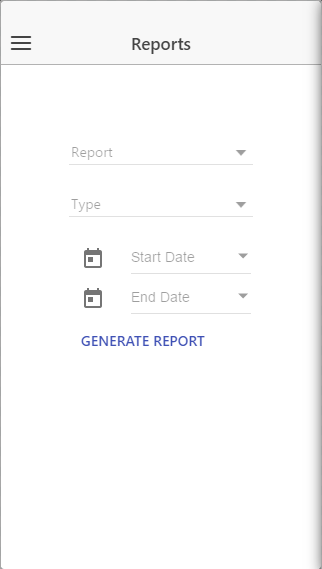
\includegraphics[width=0.15\textwidth]{Report.png}}
\end{figure}


\section{Prototyp Beschreibung}
\subsection{Side Panel}
Eine Ausstattung unserer Finanzapplikation mit einem Side Panel wurde  während der Entwicklung des low fidelity Prototyps bei den Testern durch Interviews sehr gut bewertet.\\\\Daher entschieden wir uns für die Implementierung dieses modernen Features, der dazu beiträgt, schnell zwischen verschieden Seiten zu wechseln und dabei die Übersicht zu behalten.
Damit erreichen wir eine erhöhter Benutzerfreundlichkeit unserer Applikation. Folgende Seiten sind aus Side Panel erreichbar:

\begin{itemize}
\item Einnahmen (Income)
\item Ausgaben (Expense)
\item Sparziel (Saving Target)
\item Berichte (Reports)
\item Profile (Profiles)
\end {itemize}



\subsection{Startseite der Applikation / Expense}

Auf der Startseite unserer Finanz-Applikation haben wir die Funktion "Ausgabe" implementiert, die sich während der Evaluierung unseres Prototyps als wichtigste und am öftesten zum Einsatz kommende Funktion herausgefiltert hat. 
Folgende Eingabefelder sind auf der Ausgaben-Seite möglich: 

\begin{itemize}
\item Payment Type: In der Drop-Down-Liste dieses Feldes befinden sich die unterschiedlichen Bezahl-Möglichkeiten wie Kreditkarte, Bankomat und Bar.\\
\item How much?: Eingabe von Ausgabenhöhe, das als Pflichtfeld eine Eingabe erfordert. Fehlen dieser Eingabe verhindert das Speichern der Daten. \\
\item What did you buy?: Hier gibt man den Grund der Ausgabe ein.\\
\end {itemize}

Anschließend wählt man das Ausgabendatum durch Selektion aus dem Kalenderfeld ein und speichert die Daten mit einem Klick auf das Aktionsbutton "Save" oder man löscht alle Eingaben mit "Clear" und kann die Eingabe erneut starten.  \\\\Die Selektion des Kalenderfeldes auf diese von uns implementierte Art und Weise war das Ergebnis unserer Entscheidung, die wir während unserer Interview festgestellt haben. Das trägt zu einem besseren Usability bei.


\subsection{Reports}

Eine weitere Funktion ist  der Berichtfunktion. Wie auch in der Abbildung gezeigt, hat man die Möglichkeit Ausgaben durch Auswahl eines gewünschten Diagramms/einer Tabelle und mit der Festlegung der Zeitfenster (Anfang- und Enddatum) zu visualisieren. \\Folgende Berichtstypen unter Drop-Down Liste stehen zur Verfügung: Table, Pie Chart, Area Chart, Bar Chart und Line Chart.


\subsection{Income}

Eingabe von Einkommen wurde genau so wie die Eingabe von Ausgaben möglichst einfach und verständlich gehalten, damit die Benutzer bei der Verwendung der Applikation ohne große Mühe und wenig Zeiteinsetzung gewünschte Interaktionen führen können.  \\\\Auf der Seite vom "Income" ist die Wahl des Einkommens unter Drop-Down-Liste der Einkommenstyp möglich. Einkommen wurde als Gehalt/Lohn, Forderungen und andere untergliedert. Einkommenshöhe ist ein erforderliches um die eingegebene Daten anschließend zu speichern. Das Datum kann wie bei der Aufgabenfunktion aus dem Kalenderfeld ausgewählt werden.
\clearpage

\begin{figure}
\centering
\subfigure[Side Panel]{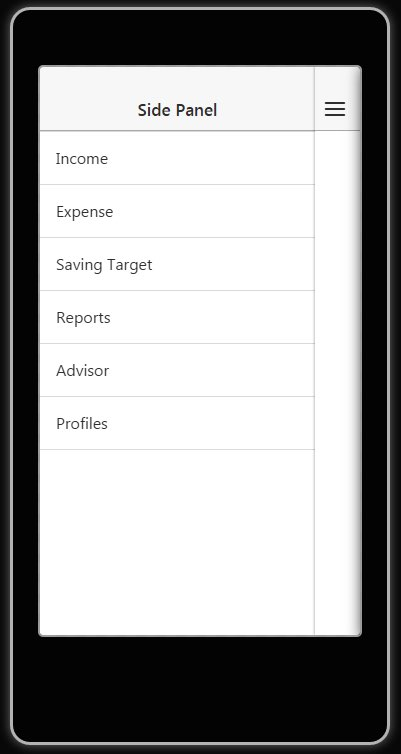
\includegraphics[width=0.15\textwidth]{sidepanel.png}}
\hfill
\subfigure[Expense]{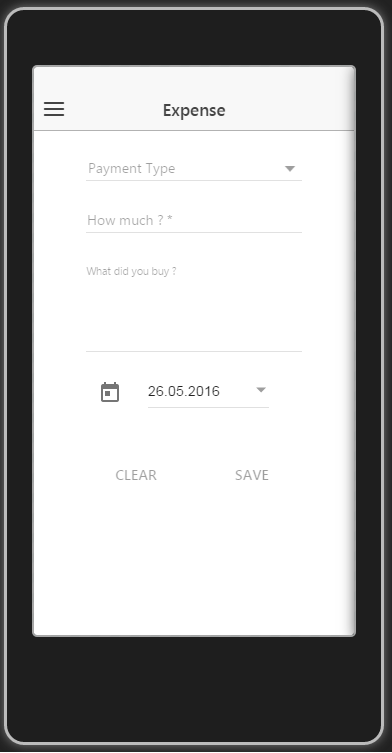
\includegraphics[width=0.15\textwidth]{expense1.png}}
\hfill
\subfigure[Report]{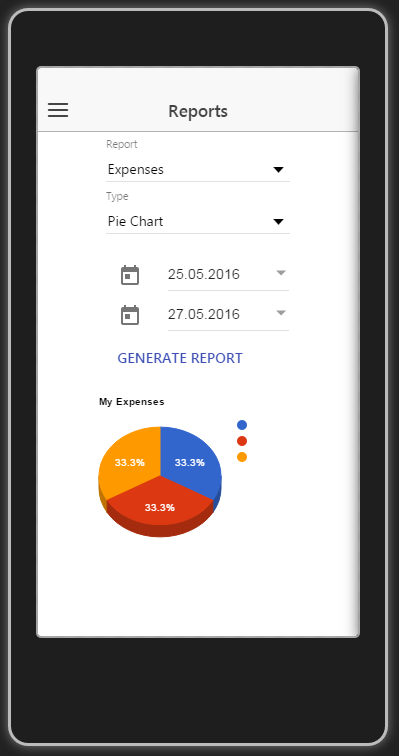
\includegraphics[width=0.15\textwidth]{reports.png}}
\hfill
\subfigure[income]{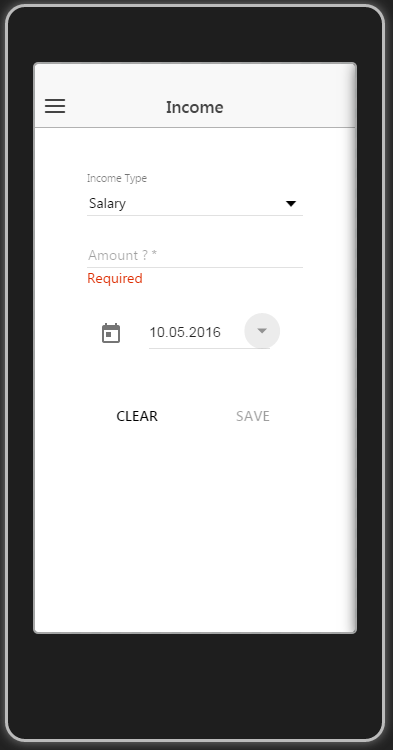
\includegraphics[width=0.15\textwidth]{income1.png}}
\end{figure}


\subsection{Technische Designentscheidungen}

Nachdem wir auch einige andere Frameworks getestet haben, darunter JQuery Mobile, entschieden wir uns letztendlich uns für AngularJS und dem Ionic Framework.\\\\ Obwohl unserer Meinung nach auch Ionic als Mobile Framework auch nicht gerade optimal ist, wird das dennoch durch die sehr gute Struktur und Verwendbarkeit von AngularJs ausgeglichen. Dank AngularJS konnten wir auch die Funktionalitäten und das Design nochmals mit dem MaterialJs Framwork erweitern, welches uns insbesondere bei den Formerstellungen eine große Hilfe.\\\\ Bezüglich des Designs haben wir auch Bootstrap verwendet, mussten aber aufgrund von Inkompatibilität, es wieder rausnehmen. \\\\ Für den Reports Bereich haben wir uns, nach einiger Recherche, für GoogleCharts entschieden und können dies auch besten Gewissens weiterempfehlen, da es unserer Meinung nach sehr leicht integrierbar ist und zugleich auch sehr detaillierte Ergebnisse liefert. Für die Speicherung der Daten würde uns eine local storage (oder auch indexeddb) nicht ausreichen.\\\\ Deshalb haben wir uns für eine SQLLite Datenbank entschieden die auch bei komplexeren Abfragen unsere App abdecken wird. 

\begin{thebibliography}{1}
\bibitem{proceeding1} http://www.color-blindness.com/coblis-color-blindness-simulator/
\end{thebibliography}


\end{document}